% Author: Grayson Orr
% Course: IN721: Mobile Application Development

\documentclass{article}
\author{}

\usepackage{graphicx}
\usepackage{wrapfig}
\usepackage{enumerate}
\usepackage{hyperref}
\usepackage[margin = 2.25cm]{geometry}
\usepackage[table]{xcolor}
\usepackage{fancyhdr}
\hypersetup{
  colorlinks = true,
  urlcolor = blue
}
\setlength\parindent{0pt}
\pagestyle{fancy}
\fancyhf{}
\rhead{College of Engineering, Construction and Living Sciences\\Bachelor of Information Technology}
\lfoot{Practical 04: Country API\\Version 1, Semester One, 2020}
\rfoot{\thepage}

\begin{document}

\begin{figure}
    \centering
    
\includegraphics[width=50mm]{./img/logo.png}
\end{figure}

\title{College of Engineering, Construction and Living Sciences\\Bachelor of Information Technology\\IN721: Mobile Application Development\\Level 7, Credits 15\\\textbf{Practical 04: Country API}}
\date{}
\maketitle

\section*{Assessment Overview}
In this assessment, you will design, develop \& UI test an application which makes a request to the \textbf{Country API} hosted on \textbf{GitHub Gist} \& displays the data using a \textbf{RecyclerView}. This assessment contributes \textbf{3\%} towards your final mark in \textbf{IN721: Mobile Application Development}.

\section*{Learning Outcomes}
At the successful completion of this course, learners will be able to: 
\begin{enumerate}
	\item Implement \& publish complete, non-trivial, industry-standard mobile applications following sound architectural \& code-quality standards.
	\item Identify relevant use cases for a mobile computing scenario \& incorporate them into an effective user experience design.
	\item Follow industry standard software engineering practice in the design of mobile applications.
\end{enumerate} 

\section*{Assessment Table}
\renewcommand{\arraystretch}{1.5}
\begin{tabular}{|l|l|l|l|l|}
	\hline      
	\vtop{\hbox{\strut \textbf{Assessment}}\hbox{\strut \textbf{Activity}}} & \textbf{Weighting} & \vtop{\hbox{\strut \textbf{Learning}}\hbox{\strut \textbf{Outcomes}}} & \vtop{\hbox{\strut \textbf{Assessment}}\hbox{\strut \textbf{Grading Scheme}}} & \vtop{\hbox{\strut \textbf{Completion}}\hbox{\strut \textbf{Requirements}}} \\
	                            
	\hline
	                                
	\small Practical                                          & \small 20\%        & \small 2, 3                                                         & \small CRA                                                                    & \small Cumulative                                                           \\ \hline  
	\small Project                                                             & \small 80\%        & \small 1, 2, 3                                                       & \small CRA                                                                    & \small Cumulative                                                           \\ \hline 
\end{tabular}

\section*{Conditions of Assessment}
You will complete this individual assessment inside \& outside timetabled class time. This assessment will need to be completed by \textbf{Friday, 16 April 2021} at \textbf{5:00 PM}. 

\section*{Pass Criteria}
This assessment is criterion-referenced (CRA) with a cumulative pass mark of \textbf{50\%} over all assessments in \textbf{IN721: Mobile Application Development}.

\section*{Authenticity}
All parts of your submitted assessment must be completely your work \& any references must be cited appropriately including, externally-sourced graphic elements. Provide your references in a \textbf{README.md} file. All media must be royalty free (or legally purchased) for educational use. Failure to do this will result in a mark of \textbf{zero} for this assessment.

\section*{Policy on Submissions, Extensions, Resubmissions \& Resits}
The school's process concerning submissions, extensions, resubmissions \& resits complies with \textbf{Otago Polytechnic} policies. Learners can view policies on the \textbf{Otago Polytechnic} website located at \href{https://www.op.ac.nz/about-us/governance-and-management/policies}{https://www.op.ac.nz/about-us/governance-and-management/policies}.

\section*{Submissions}
You must submit all program files via \textbf{GitHub Classroom}. Here is the URL to the repository you will use for your submission – \href{https://classroom.github.com/a/VJIq7Ae0}{https://classroom.github.com/a/VJIq7Ae0}. Create a new branch called  \textbf{04-country-api} from the \textbf{main} branch by running the command - \textbf{git checkout -b 04-country-api}. This branch will be your development branch for this assessment. Once you have completed this assessment, create a pull request \& assign the \textbf{GitHub} user \textbf{grayson-orr} to a reviewer. \textbf{Do not} merge your own pull request. Late submissions will incur a \textbf{10\% penalty per day}, rolling over at \textbf{5:00 PM}.

\section*{Extensions}
Familiarise yourself with the assessment due date. If you need an extension, contact the course lecturer before the due date. If you require more than a week's extension, a medical certificate or support letter from your manager may be needed.

\section*{Resubmissions}
Learners may be requested to resubmit an assessment following a rework of part/s of the original assessment. Resubmissions are to be completed within a negotiable short time frame \& usually must be completed within the timing of the course to which the assessment relates. Resubmissions will be available to learners who have made a genuine attempt at the first assessment opportunity \& achieved a \textbf{D grade (40-49\%)}. The maximum grade awarded for resubmission will be \textbf{C-}.

\section*{Resits}
Resits \& reassessments are not applicable in \textbf{IN721: Mobile Application Development}.

\section*{Instructions - Learning Outcomes 2, 3}
\subsection*{Task One (2\%):}
Create a new project with the following configurations:
\begin{itemize}
	\item Template - Empty activity
	\item Name - CountryAPI
	\item Package name - op.mobile.app.dev.country.api
	\item Save location - /path to your practical GitHub repository/04-country-api
	\item Language - Kotlin
	\item Minimum SDK - API 28: Android 9.0 (Pie) 
\end{itemize} 

The application structure is similar to the code examples from the \textbf{13-recycler-view} teaching session. Instead, you will request data from the \textbf{Country API}. \\

Familiarise yourself with the following \textbf{API} URL: \\

\href{https://gist.githubusercontent.com/Grayson-Orr/34991fb3b0192aaf636e56623cbdd9d3/raw/7e63d91a981c004a1389e7b09455336596c306d9/countries.json}{https://gist.githubusercontent.com/Grayson-Orr/34991fb3b0192aaf636e56623cbdd9d3/raw/7e63d91a981c004a1389e7b09455336596c306d9/countries.json} \\

In \textbf{recycler\_view\_item.xml}, add two \textbf{TextViews} \& an \textbf{ImageView}. You will bind your model data to these \textbf{Views}. However, binding data to an \textbf{ImageView} is not quite straight forward.  \\

\textbf{Glide} is a fast \& efficient image loading framework that supports fetching \& displaying images. To use \textbf{Glide}, declare the following dependency in \textbf{build.gradle (CountryAPI.app)}.

\begin{verbatim}
dependencies {
    ...
    implementation 'com.github.bumptech.glide:glide:4.8.0'
    ...
}
\end{verbatim}

In \textbf{ServiceStatusBindingAdapter.kt}, add the following \textbf{BindingAdapter} function:

\begin{verbatim}
    ...

    @BindingAdapter("flagImage")
    fun bindFlagImage(imageView: ImageView, imageUrl: String) {
        Glide.with(view.context)
            .load(imageUrl).apply(RequestOptions().circleCrop())
            .into(view)
    }
\end{verbatim}

\textbf{Resource:} \href{https://github.com/bumptech/glide}{https://github.com/bumptech/glide} \\

In \textbf{recycler\_view\_item.xml}, declare \& set the \textbf{flagImage} attribute to the flag image data in your model. \\

Run your application on either an \textbf{Android Emulator} or \textbf{connect device}. \\ 

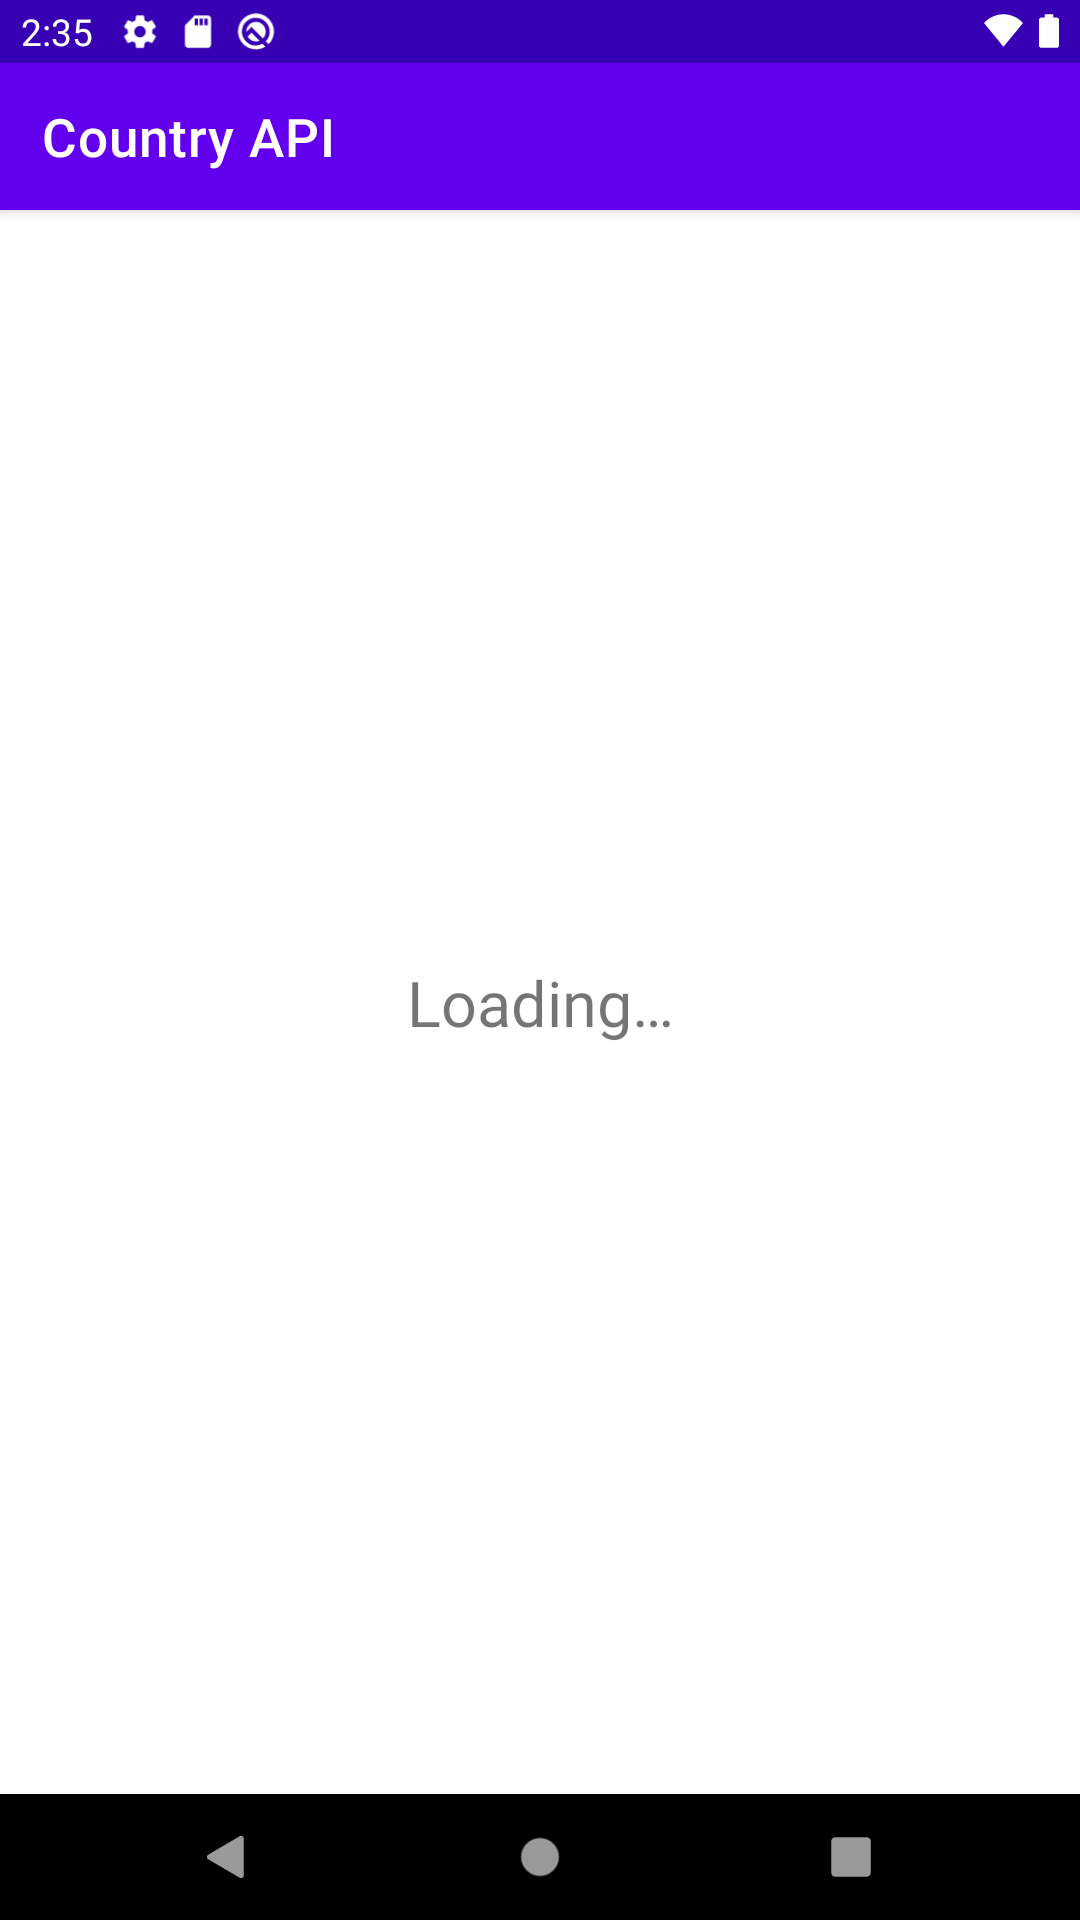
\includegraphics[width=5cm, height=9cm]{../tex/img/practicals/04-country-api-1.png} 
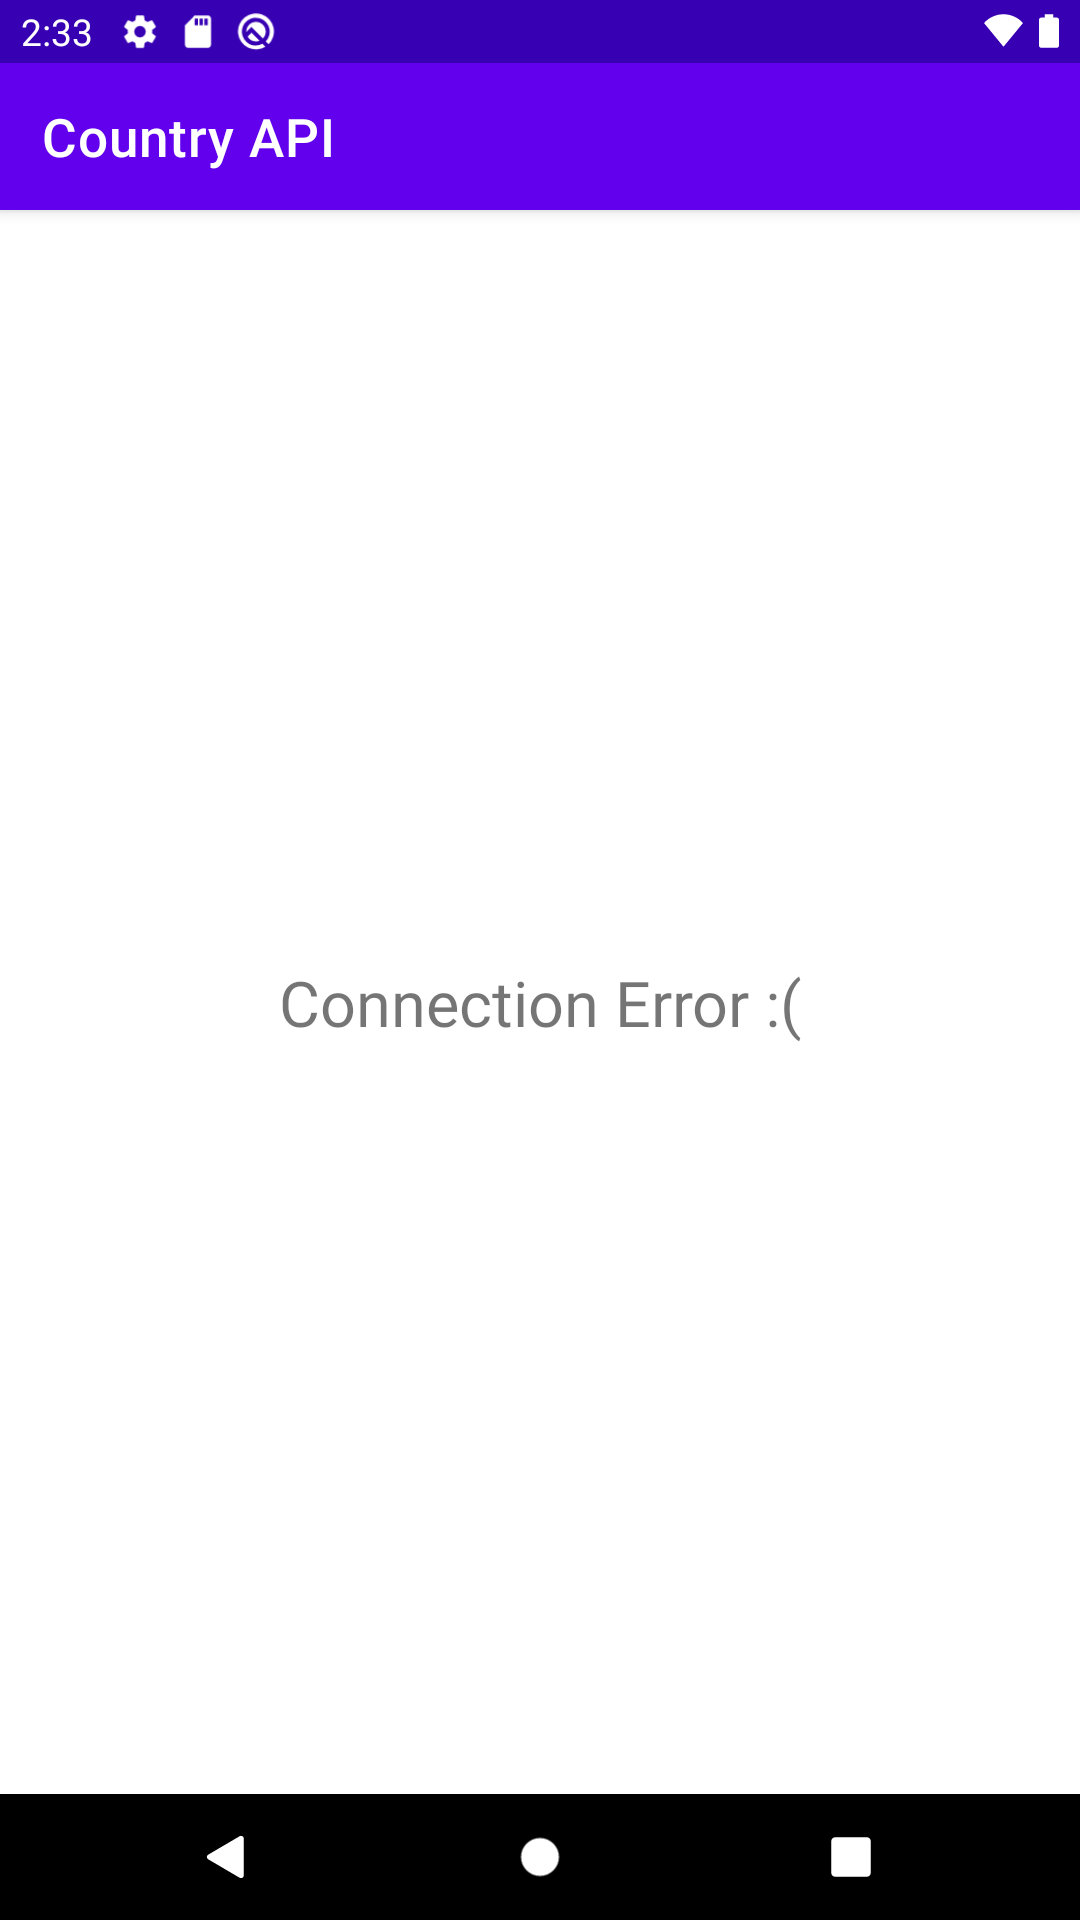
\includegraphics[width=5cm, height=9cm]{../tex/img/practicals/04-country-api-2.png}
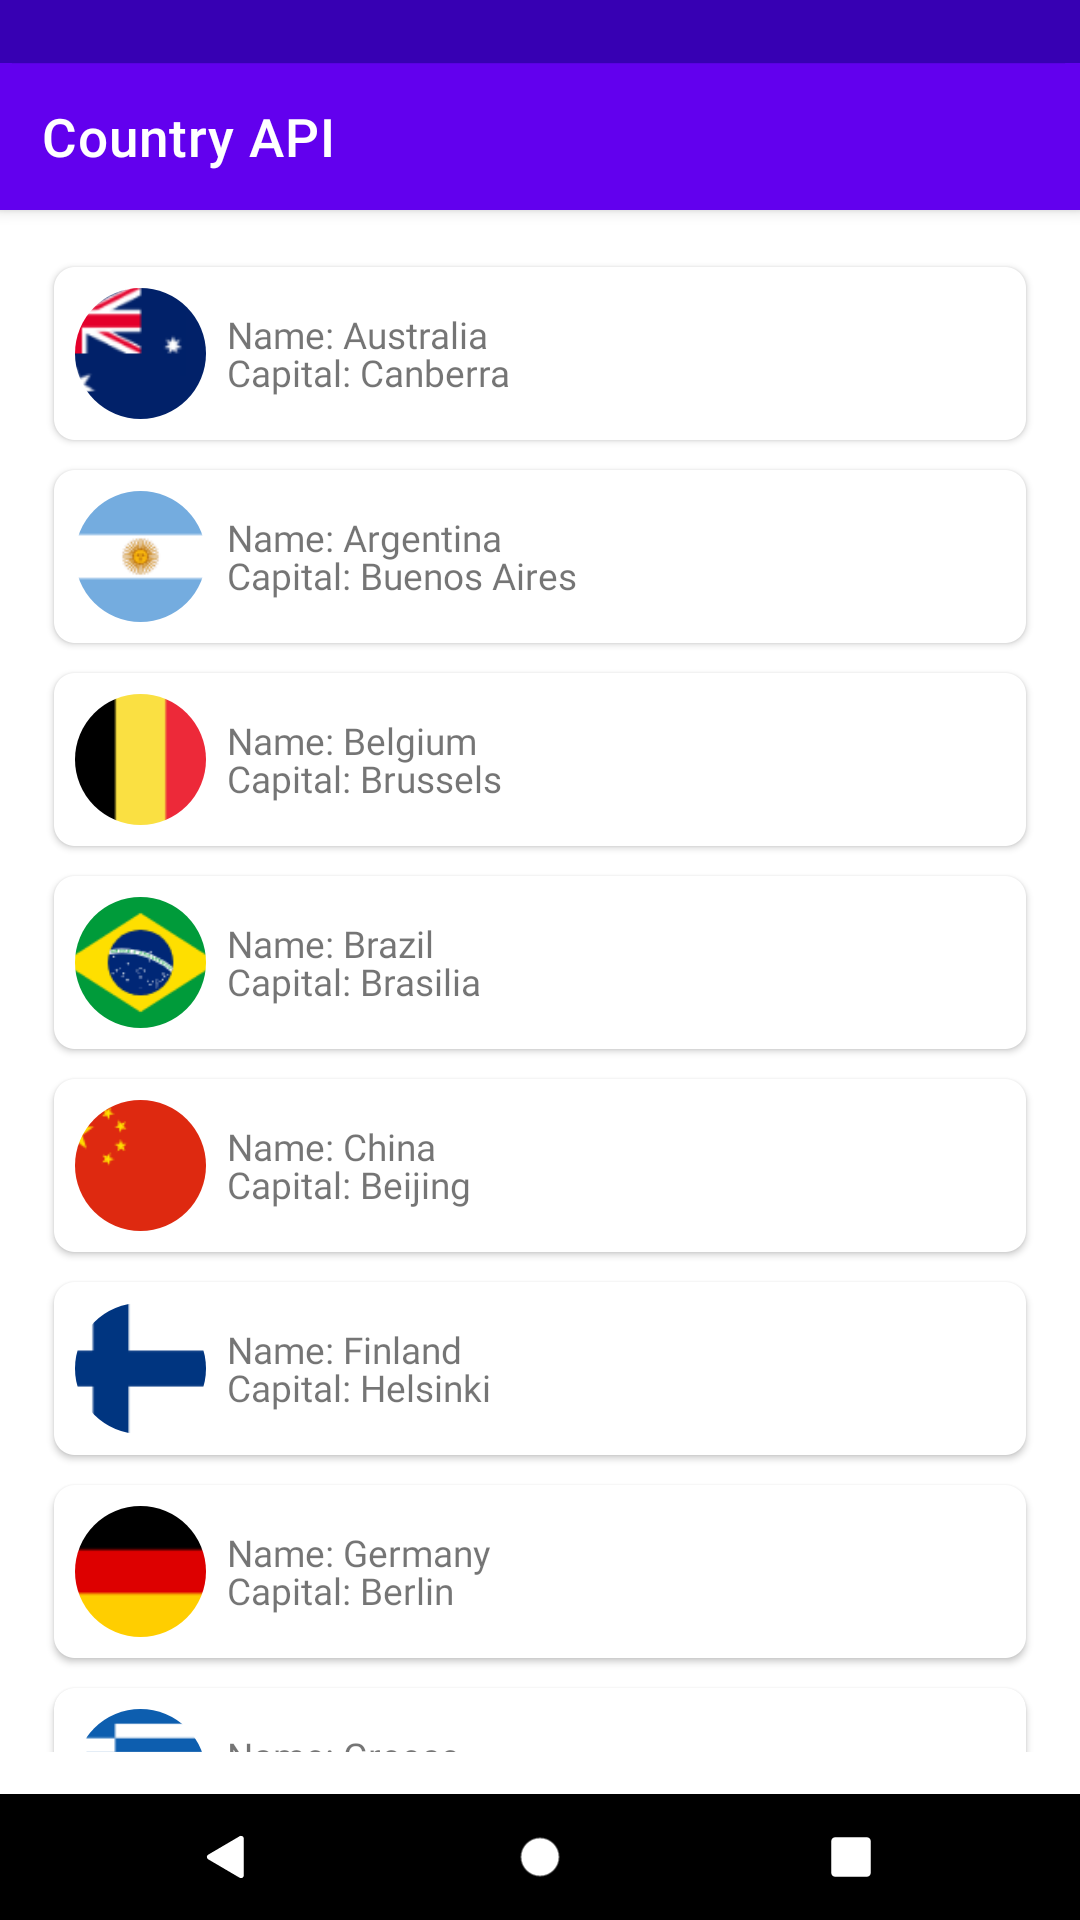
\includegraphics[width=5cm, height=9cm]{../tex/img/practicals/04-country-api-3.png} \\

\subsection*{Task Three (1\%):}
Create a new test file called \textbf{CountryTest}. To do this, right-click on \textbf{op.mobile.app.dev.country (androidTest) $>$ Kotlin Class/File}. In \textbf{CountryTest.kt}, write three UI tests. To run your test file, right-click \textbf{CountryTest.kt $>$ 'Run CountryTest'}.

\end{document}